

\hypertarget{sec:plane-solutions}{%
\subsection{Planar Response of Cantilever Beam Under End Moment and End Force}\label{sec:plane}}
\begin{figure}[h]
\centering
\begin{subfigure}[b]{0.48\textwidth}
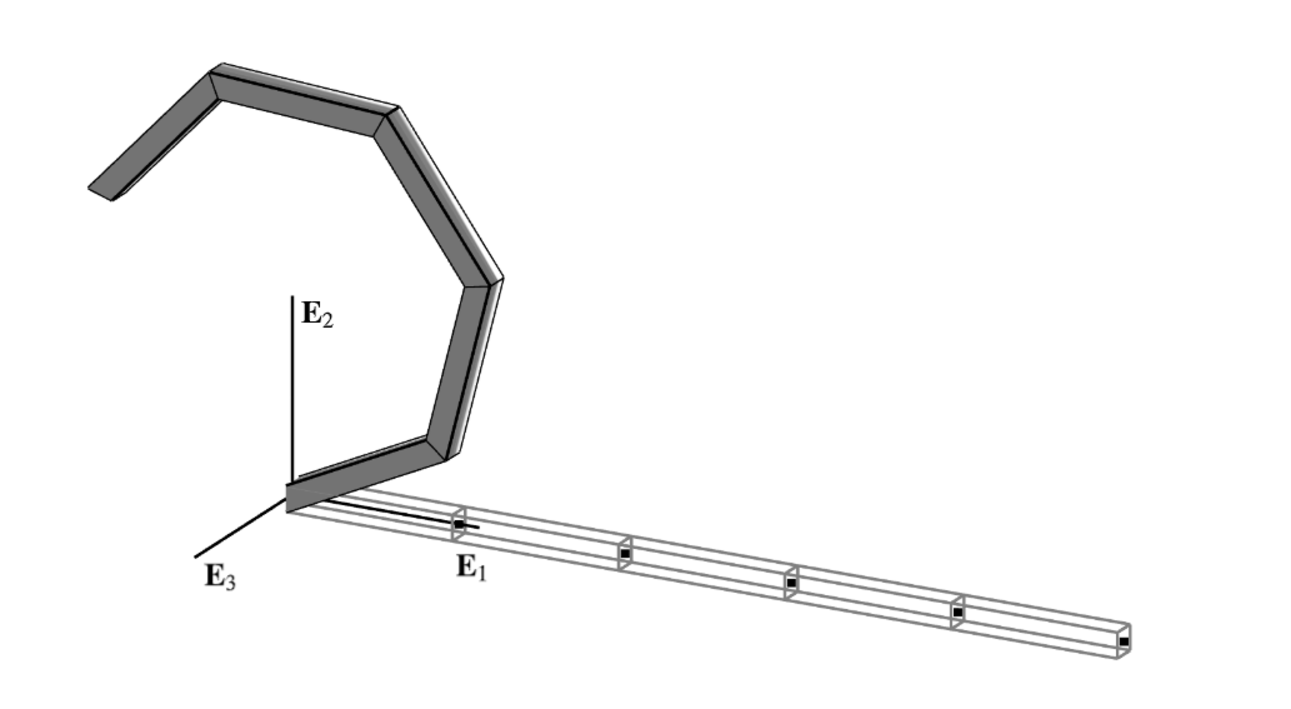
\includegraphics[width=0.8\textwidth,keepaspectratio]{Figures/Figure_1a}
  \caption{\(\lambda = 0.7\)}
  \label{fig:helical-a}
\end{subfigure}
\begin{subfigure}[b]{0.48\textwidth}
  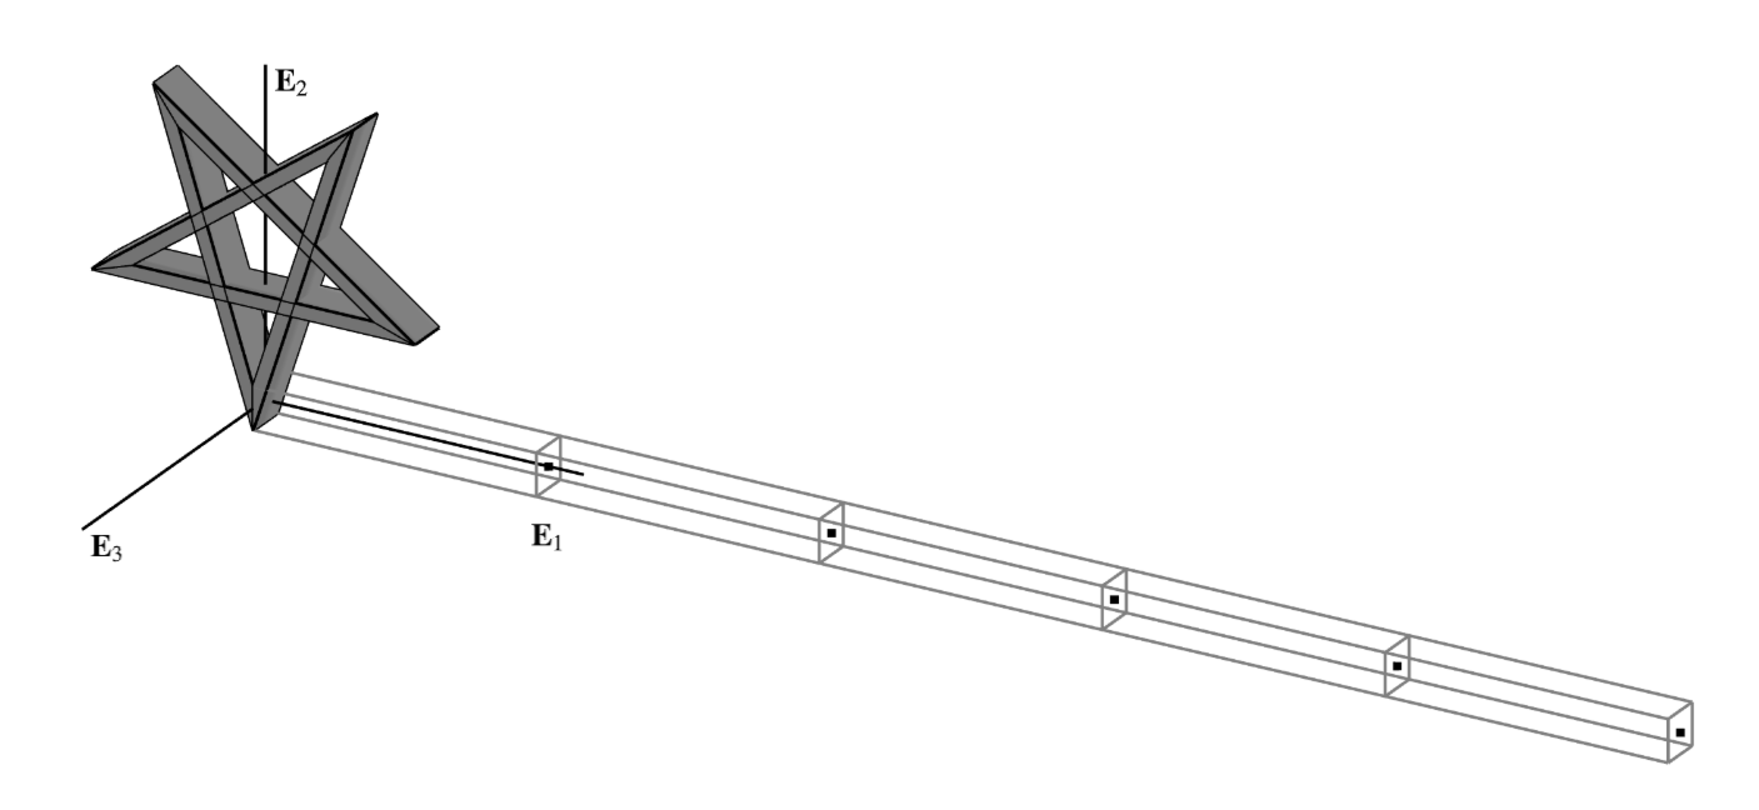
\includegraphics[width=0.8\textwidth,keepaspectratio]{Figures/Figure_1b}
  \caption{\(\lambda = 2\)}
  \label{fig:helical-b}
\end{subfigure}
\caption{Deformed configuration of cantilever beam under two moment magnitudes.} %end moment scale factor of \(\lambda=0.7\) (\ref{fig:helical-a}) and \(\lambda=2\) (b).}
\label{fig:cantilever}
\end{figure}
%
The cantilever beam 
in Figure \ref{fig:cantilever} is subjected to \emph{either} a point moment \(\boldsymbol{M}\) 
or a point force \(F \, \mathbf{E}_3\) at its free end \(\reflenx=L\).
%
The centerline of the reference configuration 
is given by \(\boldsymbol{x}_0(\reflenx) = \reflenx\,\mathbf{E}_1\).
This example is selected to demonstrate the ability of the proposed formulations to accurately reproduce available analytical solutions.
%
\subsubsection{End Moment}\label{sec:circle}
%
%
When \(F = 0\) the configuration is expected
to remain in the \(\mathbf{E}_1 - \mathbf{E}_2\) plane.
Consequently, the out-of-plane director
\(\mathbf{D}_3\) does not change during deformation so that \(\mathbf{d}_3 = \mathbf{D}_3\).
This simplification has two important consequences:
\begin{itemize}
  \item There is no distinction between a spatially applied moment \(\boldsymbol{M} = M \, \mathbf{d}_3\)
    and a materially applied moment \(\boldsymbol{M} = M \, \mathbf{D}_3\).
  \item The rotation \(\boldsymbol{\Lambda}\) becomes
    vectorial, its variations \(\boldsymbol{u}_{\scriptscriptstyle{\Lambda}}^{(i)}\) at different configurations \(\chi^{(i)}\) can be added, and the sum of these variations over the course of global equilibrium iterations is equivalent
    to the logarithmic rotation increment:
    \[
      \sum_{i=0}^n \boldsymbol{u}_{\scriptscriptstyle{\Lambda}}^{(i)} \equiv \boldsymbol{\theta} 
     = \operatorname{Log} \left(\boldsymbol{\Lambda}_{(n)}\boldsymbol{\Lambda}_{(0)}^{\mathrm{t}}\right).
    \]
    %This is because the plane constraint has rendered the configuration manifold for \(\boldsymbol{\Lambda}\) vectorial.
\end{itemize}
%
In this case, the moment loading can be treated identically for all analyses by simply scaling a constant \emph{reference} force vector for the node at \(\reflenx=L\):
%
\begin{equation}
  \mathbf{f}_{M,\text{ref}} = \begin{pmatrix}
     0 & 0 & M
  \end{pmatrix}^{\mathrm{t}}
  \label{eq:fref}
\end{equation}
%
where the reference magnitude \(M = \lambda 2 \pi EI/L \) varies with $\lambda=1/8, \ 1$, and $2$ for different cases causing the cantilever to loop over itself \(\lambda\) times. 
The following parameters are used:
\[
\begin{array}{lcr}
    L  &=&    10\hphantom{..}    \\ % ,& A  &= 1 \\
    E  &=&    10^4  \\ % ,& I  &= 10^{-2} \\
    G  &=&    10^4  \\ % ,& J  &= 10^{-2} \\
\end{array}
\qquad\qquad
\begin{array}{lcr}
    A  &=& 1\hphantom{..} \\
    I  &=& 10^{-2} \\
    J  &=& 10^{-2} \\
\end{array}
\]
The simulation uses a \emph{single} load step with uniform meshes of 5 and 10 elements for the  2-node and 3-node
variants of all formulations in Table~\ref{tab:variants}. 
%
The solution requires only two iterations for each formulation matching the ideal performance reported by \cite{simo1986threedimensional}.
The tip displacements for the case \(\lambda = 1/8\) are collected in Table~\ref{tab:helical-plane} along with
the analytic solution of the governing boundary value problem in Equation~(\ref{eq:strong}) given by:
\begin{equation*}
  \left\{
  \begin{aligned}
  \bm{x}(\reflenx)&=\frac{EI}{M} \sin \vartheta(\reflenx) \, \mathbf{E}_1
                      + \frac{EI}{M}\left(\cos \vartheta(\reflenx)-1\right) \, \mathbf{E}_2 \\
    \vartheta(\xi)   &=  \reflenx \frac{M}{EI}
  \end{aligned}
  \right.
\end{equation*}
%
where \(\vartheta\) parameterizes the rotation \(\boldsymbol{\Lambda}(\reflenx) = \operatorname{Exp} \vartheta(\reflenx) \, \mathbf{E}_3\). This result is derived in Appendix~\ref{sec:closed-solution}. 
The displacements for \(n=2\)-node elements match exactly those reported by \cite{ibrahimbegović1995computational} for both the natural \texttt{None}, and the logarithmic \texttt{Init}/\texttt{Incr} variants.
For \(n=3\)-node elements, the results match the analytic solution up to the reported precision.
%
%
\begin{center}
\begin{table*}[H]%
  \caption{Tip displacements for the helical cantilever beam under $\lambda = 1/8$ for a discretization with 10 \(n\)-node elements.}
\label{tab:helical-plane}

% indicating agreement with exact solution (at M=2.75*loops, 2-nodes)

% indicating agreement with referenced formulations (at M=2.5, F=0.0625, 2-nodes)


\begin{tabular*}{\textwidth}{@{\extracolsep\fill}cccccccc@{}}
\toprule
\textbf{Interpolation} & \textbf{Isometry}  & \textbf{Parameters} & 
\(n\)  & \(\Delta x_1\) & \(\Delta x_2\) & \(\Delta x_3\)  \\
\midrule
% \texttt{None} & \texttt{None} & \texttt{None} & 2  & -0.994522 & 3.73019 & 0 \\
  \texttt{None} & \texttt{SFIN} & \texttt{None} & 2  & -0.994522 & 3.73019 & 0 \\
% \texttt{Incr} & \texttt{None} & \texttt{Incr} & 2  & -0.994522 & 3.73019 & 0 \\
  \texttt{Incr} & \texttt{SFIN} & \texttt{Incr} & 2  & -0.994522 & 3.73019 & 0 \\
% \texttt{Init} & \texttt{None} & \texttt{Init} & 2  & -0.994522 & 3.73019 & 0 \\
% \texttt{None} & \texttt{SFIN} & \texttt{Incr} & 2  & -0.994522 & 3.73019 & 0 \\
  \texttt{Incr} & \texttt{SFIN} & \texttt{None} & 2  & -0.994522 & 3.73019 & 0 \\
% \texttt{None} & \texttt{None} & \texttt{Incr} & 2  & -0.994522 & 3.73019 & 0 \\
%
  \hline
  \texttt{None} & \texttt{SFIN} & \texttt{None} & 3 & -0.996837 & 3.72923 & 0 \\
  \texttt{Incr} & \texttt{SFIN} & \texttt{Incr} & 3 & -0.996837 & 3.72923 & 0 \\ %-6.66134e-16
  \texttt{Incr} & \texttt{SFIN} & \texttt{None} & 3 & -0.996837 & 3.72923 & 0 \\ % -1.11022e-15 \\
\midrule
\textbf{Analytic} &             &               &   & \textbf{-0.996837} & \textbf{3.72923} & \textbf{0} \\ %-6.66134e-16
\hline
\end{tabular*}

\end{table*}
\end{center}
%
%
\subsubsection{End Force}\label{sec:elastica}
% \begin{figure}
% \centering
% \includegraphics[width=0.6\textwidth,keepaspectratio]{Figures/Buckling_2}
% \caption{.}
% \end{figure}
% This example investigates the response of the cantilver for a more complicated analytic planar solution.
In this case the cantilever beam is subjected only to a transverse force of \(\boldsymbol{F} = 10 \, \mathbf{E}_2\) in a single step. 
The simulation uses the following geometric and material properties from the literature:
\[
\begin{array}{lr}
L  =&    1 \\
E  =&   10 \\
\hphantom{.}
% G  =   GAv/A
\end{array}
\qquad 
\begin{array}{lr}
A  =&   10^7 \\
I  =&    1   \\
J  =&   10^7 \\
\end{array}
\]
Two values for the shear modulus \(G\) are used with a shear stiffness \(GA\) of \(500\) and \(10\), respectively, the latter representing the case with significant shear deformations. 
Table~\ref{tab:transv} presents the numerical tip displacements and the analytic solution from \cite{batista2016closedform} using Jacobi elliptic functions and accounting for flexural and shear deformations.
%
The analysis uses both 2-node and 4-node elements.
For the sake of brevity, the results are reported only for the variants using
the same parameterization as the wrapped element's interpolation.
%
\begin{center}
\begin{table*}%[ht]%
\caption{Tip displacements for transversely loaded plane cantilver.}
\label{tab:transv}

\begin{tabular*}{\textwidth}{@{\extracolsep\fill}cccccccc@{}}
\toprule
\textbf{Interpolation}   & \textbf{Isometry} & %\textbf{Parameters} &
\(GA\) &  \textbf{Nodes}   &
\textbf{Max. Iter.} &
\(\Delta x_1\)   & \(\Delta x_2\) 
\\
\midrule
%
  \texttt{None}   &  \texttt{None} &  500   & 2 &     6 & -0.061013882  &          0.31723971 \\
  \texttt{None}   &  \Spherical{} &  500   & 2 &     6 & -0.061013882  &          0.31723971 \\
  \texttt{Incr}   &  \texttt{None} &  500   & 2 &     8 & -0.061013882  &          0.31723971 \\
  \texttt{Incr}   &  \Spherical{} &  500   & 2 &     6 & -0.061013882  &          0.31723971 \\
  \texttt{Init}   &  \texttt{None} &  500   & 2 &     8 & -0.061013882  &          0.31723971 \\
  \texttt{Init}   &  \Spherical{} &  500   & 2 &     6 & -0.061013882  &          0.31723971 \\
% \texttt{None}   &  \texttt{None} &  500   & 3 &     6 & -0.061315563  &          0.31781382 \\
% \texttt{None}   &  \Spherical{} &  500   & 3 &     6 & -0.061315563  &          0.31781382 \\
% \texttt{Incr}   &  \texttt{None} &  500   & 3 &     8 & -0.061315563  &          0.31781382 \\
% \texttt{Incr}   &  \Spherical{} &  500   & 3 &     6 & -0.061315563  &          0.31781382 \\
% \texttt{Init}   &  \texttt{None} &  500   & 3 &     8 & -0.061315563  &          0.31781382 \\
% \texttt{Init}   &  \Spherical{} &  500   & 3 &     6 & -0.061315563  &          0.31781382 \\
  \texttt{None}   &  \texttt{None} &  500   & 4 &     6 & -0.061315634  &          0.31781389 \\
  \texttt{None}   &  \Spherical{} &  500   & 4 &     6 & -0.061315634  &          0.31781389 \\
  \texttt{Incr}   &  \texttt{None} &  500   & 4 &     8 & -0.061315634  &          0.31781389 \\
  \texttt{Incr}   &  \Spherical{} &  500   & 4 &     6 & -0.061315634  &          0.31781389 \\
  \texttt{Init}   &  \texttt{None} &  500   & 4 &     8 & -0.061315634  &          0.31781389 \\
  \texttt{Init}   &  \Spherical{} &  500   & 4 &     6 & -0.061315634  &          0.31781389 \\
\midrule                                   
\textbf{Analytic} &                &        &   &&\textbf{-0.06131566}  &  \textbf{0.31781387} \\
% \hline                                   
% \texttt{None}   &  \texttt{None} &   7.0  & 2 &     7 & -0.10295637   &          0.46498401 \\
% \texttt{None}   &  \Spherical{} &   7.0  & 2 &     7 & -0.10295637   &          0.46498401 \\
% \texttt{Incr}   &  \texttt{None} &  10.0  & 2 &    10 & -0.10295637   &          0.46498401 \\
% \texttt{Incr}   &  \Spherical{} &   7.0  & 2 &     7 & -0.10295637   &          0.46498401 \\
% \texttt{Init}   &  \texttt{None} &  10.0  & 2 &    10 & -0.10295637   &          0.46498401 \\
% \texttt{Init}   &  \Spherical{} &   7.0  & 2 &     7 & -0.10295637   &          0.46498401 \\
% \texttt{None}   &  \texttt{None} &   8.0  & 3 &     8 & -0.10328482   &          0.46541329 \\
% \texttt{None}   &  \Spherical{} &   8.0  & 3 &     8 & -0.10328482   &          0.46541329 \\
% \texttt{Incr}   &  \texttt{None} &   9.0  & 3 &     9 & -0.10328482   &          0.46541329 \\
% \texttt{Incr}   &  \Spherical{} &   8.0  & 3 &     8 & -0.10328482   &          0.46541329 \\
% \texttt{Init}   &  \texttt{None} &   9.0  & 3 &     9 & -0.10328482   &          0.46541329 \\
% \texttt{Init}   &  \Spherical{} &   8.0  & 3 &     8 & -0.10328482   &          0.46541329 \\
% \texttt{None}   &  \texttt{None} &  10.0  & 4 &    10 & -0.10328489   &          0.46541332 \\
% \texttt{None}   &  \Spherical{} &  10.0  & 4 &    10 & -0.10328489   &          0.46541332 \\
% \texttt{Incr}   &  \texttt{None} &  10.0  & 4 &    10 & -0.10328489   &          0.46541332 \\
% \texttt{Incr}   &  \Spherical{} &  10.0  & 4 &    10 & -0.10328489   &          0.46541332 \\
% \texttt{Init}   &  \texttt{None} &  10.0  & 4 &    10 & -0.10328489   &          0.46541332 \\
% \texttt{Init}   &  \Spherical{} &  10.0  & 4 &    10 & -0.10328489   &          0.46541332 \\
%                 &                &        &   &&\textbf{-0.10328492}  &  \textbf{0.46541330} \\
  \hline                                   
  \texttt{None}   &  \texttt{None} &   10   & 2 &   \;8 & -0.25174992   &          1.1670173 \\
  \texttt{None}   &  \Spherical{} &   10   & 2 &   \;8 & -0.25174992   &          1.1670173 \\
  \texttt{Incr}   &  \texttt{None} &   10   & 2 &    11 & -0.25174992   &          1.1670173 \\
  \texttt{Incr}   &  \Spherical{} &   10   & 2 &   \;8 & -0.25174992   &          1.1670173 \\
  \texttt{Init}   &  \texttt{None} &   10   & 2 &    11 & -0.25174992   &          1.1670173 \\
  \texttt{Init}   &  \Spherical{} &   10   & 2 &   \;8 & -0.25174992   &          1.1670173 \\
% \texttt{None}   &  \texttt{None} &   10   & 3 &   \;8 & -0.25213654   &          1.1670959 \\
% \texttt{None}   &  \Spherical{} &   10   & 3 &   \;8 & -0.25213654   &          1.1670959 \\
% \texttt{Incr}   &  \texttt{None} &   10   & 3 &    11 & -0.25213654   &          1.1670959 \\
% \texttt{Incr}   &  \Spherical{} &   10   & 3 &   \;8 & -0.25213654   &          1.1670959 \\
% \texttt{Init}   &  \texttt{None} &   10   & 3 &    11 & -0.25213654   &          1.1670959 \\
% \texttt{Init}   &  \Spherical{} &   10   & 3 &   \;8 & -0.25213654   &          1.1670959 \\
  \texttt{None}   &  \texttt{None} &   10   & 4 &   \;8 & -0.25213659   &          1.1670959 \\
  \texttt{None}   &  \Spherical{} &   10   & 4 &   \;8 & -0.25213659   &          1.1670959 \\
  \texttt{Incr}   &  \texttt{None} &   10   & 4 &    12 & -0.25213659   &          1.1670959 \\
  \texttt{Incr}   &  \Spherical{} &   10   & 4 &   \;8 & -0.25213659   &          1.1670959 \\
  \texttt{Init}   &  \texttt{None} &   10   & 4 &    12 & -0.25213659   &          1.1670959 \\
  \texttt{Init}   &  \Spherical{} &   10   & 4 &   \;8 & -0.25213659   &          1.1670959 \\
  \midrule                                 
  \textbf{Analytic} &              &        &   &&\textbf{-0.25213661}  &  \textbf{1.1670959} \\
% \hline                                   
% \texttt{None}   &  \texttt{None} &   9.0  & 2 &     9 & -0.37576182   &          2.1041297 \\
% \texttt{None}   &  \Spherical{} &   9.0  & 2 &     9 & -0.37576182   &          2.1041297 \\
% \texttt{Incr}   &  \texttt{None} &  19.0  & 2 &    19 & -0.37576182   &          2.1041297 \\
% \texttt{Incr}   &  \Spherical{} &   9.0  & 2 &     9 & -0.37576182   &          2.1041297 \\
% \texttt{Init}   &  \texttt{None} &  19.0  & 2 &    19 & -0.37576182   &          2.1041297 \\
% \texttt{Init}   &  \Spherical{} &   9.0  & 2 &     9 & -0.37576182   &          2.1041297 \\
% \texttt{None}   &  \texttt{None} &   9.0  & 3 &     9 & -0.37612139   &          2.1040875 \\
% \texttt{None}   &  \Spherical{} &   9.0  & 3 &     9 & -0.37612139   &          2.1040875 \\
% \texttt{Incr}   &  \texttt{None} &  12.0  & 3 &    12 & -0.37612139   &          2.1040875 \\
% \texttt{Incr}   &  \Spherical{} &   9.0  & 3 &     9 & -0.37612139   &          2.1040875 \\
% \texttt{Init}   &  \texttt{None} &  12.0  & 3 &    12 & -0.37612139   &          2.1040875 \\
% \texttt{Init}   &  \Spherical{} &   9.0  & 3 &     9 & -0.37612139   &          2.1040875 \\
% \texttt{None}   &  \texttt{None} &   9.0  & 4 &     9 & -0.37612139   &          2.1040875 \\
% \texttt{None}   &  \Spherical{} &   9.0  & 4 &     9 & -0.37612139   &          2.1040875 \\
% \texttt{Incr}   &  \texttt{None} &  12.0  & 4 &    12 & -0.37612139   &          2.1040875 \\
% \texttt{Incr}   &  \Spherical{} &   9.0  & 4 &     9 & -0.37612139   &          2.1040875 \\
% \texttt{Init}   &  \texttt{None} &  12.0  & 4 &    12 & -0.37612139   &          2.1040875 \\
% \texttt{Init}   &  \Spherical{} &   9.0  & 4 &     9 & -0.37612139   &          2.1040875 \\
%\midrule                                  
% \textbf{Analytic} &              &        &   &&\textbf{-0.37612140}  &  \textbf{2.1040875} \\
%
\bottomrule
\end{tabular*}

\end{table*}
\end{center}


\iffalse
\begin{center}
\begin{table*}[hb]
\caption{Buckling with two elements in 15 steps. \texttt{Petrov=false},
\(A = 50000\) and \textbf{B2} triad.}
\begin{tabular*}{\textwidth}{@{\extracolsep\fill}llrrrr@{}}
%\begin{tabular*}[]{@{}llrrrr@{}}
\toprule
Element & Rotation & Avg. Iter & Max. Iter & \(u_t\) & Error \\
\midrule
\texttt{Elastica1D}           & Init & 4.03 & 6 & 0.775947 & 0\% \\
\texttt{LE2dFrm\_w2ndOrdFF}   & Init & 7.53 & 16 & 0.793910 & 2.3149\% \\
\texttt{DisplShear3dFrm\_wCS} & Iter & 6.13 & 9 & 0.833646 & 7.4359\% \\
\texttt{DisplShear3dFrm\_wCS} & Incr & 6.13 & 9 & 0.833646 & 7.4359\% \\
\texttt{DisplShear3dFrm\_wCS} & Init & 6.13 & 9 & 0.833646 & 7.4359\% \\
\texttt{Corot3dFrm} & Iter & 6.87 & 11 & 0.825041 & 6.3269\% \\
\texttt{Corot3dFrm} & Incr & 7.00 & 13 & 0.833647 & 7.4361\% \\
\texttt{Corot3dFrm} & Init & 7.00 & 13 & 0.833647 & 7.4361\% \\
\end{tabular*}
\end{table*}
\end{center}
\fi
